% Intended LaTeX compiler: xelatex
\documentclass[aspectratio=64,12pt]{beamer}
\usepackage{graphicx}
\usepackage{longtable}
\usepackage{wrapfig}
\usepackage{rotating}
\usepackage[normalem]{ulem}
\usepackage{amsmath}
\usepackage{amssymb}
\usepackage{capt-of}
\usepackage{hyperref}
\institute{Università di Siena}
\usepackage{localheader}
\usepackage{tikz}
\usepackage{booktabs,tabularx}
\usepackage{setspace}
\usepackage{quoting}
\usepackage[italian]{babel}
\usepackage{fancybox}
\newcolumntype{R}{>{\raggedleft\arraybackslash}X}
\usetheme{default}
\author{Massimo D'Antoni}
\date{2024-2025}
\title{Le imposte}
\subtitle{Scienza delle Finanze}
\hypersetup{
 pdfauthor={Massimo D'Antoni},
 pdftitle={Le imposte},
 pdflang={Italian}}
\begin{document}

\maketitle

\section{Una visione di insieme}

%%%%%%%%%%%%%%%%%%%%%%%%%%%%%%%%%%%%%%%%%%%%%%%%%
\begin{frame}{Classificazione delle imposte}
Nel Conto consolidato delle pubbliche amministrazioni le entrate correnti si distinguono in:
% DATI ISTAT Conto economico per sottosettore
% Conti nazionali > Conti e aggregati economici delle Pubbliche Amministrazioni >
% Conto annuale

\begin{table}[H]\footnotesize
\begin{tabularx}{\linewidth}{lRRR}
    \toprule
  ENTRATE &miliardi di €&\% PIL &\% Entrate\tabularnewline
  \midrule
Produzione vendibile e per uso proprio &49,6  &2,4  &5,0\tabularnewline
Imposte indirette  &294,7  &14,1  &29,6\tabularnewline
Imposte dirette  &320,8  &15,4  &32,2\tabularnewline
Contributi sociali  &269,2  &12,9  &27,0\tabularnewline
Altre entrate correnti  &35,2  &1,8  &3,8\tabularnewline
\midrule
Entrate correnti  &972,6  &46,6  &97,6\tabularnewline
Entrate in c/capitale  &23,9  &1,1  &2,4\tabularnewline
\midrule
Totale entrate  &996,6  &47,8  &100,0\tabularnewline
\bottomrule
\multicolumn{4}{r}{Dati ISTAT. Anno: 2023}
\end{tabularx}
\end{table}
\end{frame}


%%%%%%%%%%%%%%%%%%%%%%%%%%%%%%%%%%%%%%%%%%%%%%%%%
\begin{frame}{Classificazione nella contabilità nazionale}
\begin{itemize}
\item \emph{Tax} = prelievi operati dalle P.A
\begin{itemize}
\item obbligatori (\emph{compulsory})
\item senza corrispettivo (\emph{unrequited}), «unilaterali»
\end{itemize}
Si traduce a seconda dei casi con \alert{imposte} e \alert{tasse}
\item \alert{Imposte dirette} = pagamenti periodici su reddito e patrimonio
\item \alert{Imposte indirette} = prelievi su produzione e importazione di beni e
servizi, su utilizzazione del lavoro, sulla proprietà di terreni e
fabbricati e su altri beni impiegati nella produzione
\item \alert{Contributi sociali} = versamenti a enti previdenziali per prestazioni
pensionistiche e assicurative
\begin{itemize}
\item Prevedono un legame più diretto tra versamenti e diritto alla prestazione
o ammontare della prestazione
\end{itemize}
\item \alert{Produzione vendibile} = proventi da beni e servizi destinati alla vendita
\item \alert{Redditi di capitale} = dividendi da partecipazioni e altro
\end{itemize}
\end{frame}

%%%%%%%%%%%%%%%%%%%%%%%%%%%%%%%%%%%%%%%%%%%%%%%%%
\begin{frame}{Classificazione «tradizionale» italiana}
La classificazione «tradizionale» italiana presenta alcune differenze:
\begin{itemize}
\item Le \alert{imposte dirette} colpiscono manifestazioni immediate della
  capacità contributiva quali la percezione di un reddito o il possesso di un
  patrimonio. Si usa distinguerle a loro volta in
\begin{itemize}
\item imposte \alert{personali}, il cui ammontare dipende da caratteristiche
soggettive del contribuente (ad es. livello complessivo del reddito,
condizione familiare);
\item imposte \alert{reali}, il cui ammontare dipende solo dall'oggetto dell'imposta
(categoria di reddito o patrimonio).
\end{itemize}
\item le \alert{imposte indirette} colpiscono manifestazioni mediate della capacità
contributiva, quali il consumo o scambio di un bene o servizio o il
trasferimento di una proprietà patrimoniale.
\item le \alert{tasse} sono tributi corrisposti a fronte di un bene/servizio di cui beneficiano il richiedente e la collettività (es. tasse scolastiche).
\end{itemize}

\begin{block}{}
Nella classificazione italiana, che ritroviamo in molti documenti ufficiali anche di carattere normativo, sono considerate imposte dirette l'IMU e l'IRAP.
\end{block}
\end{frame}

%%%%%%%%%%%%%%%%%%%%%%%%%%%%%%%%%%%%%%%%%%%%%%%%%
\begin{frame}{Composizione della pressione fiscale}
\begin{figure}[htbp]
\centering
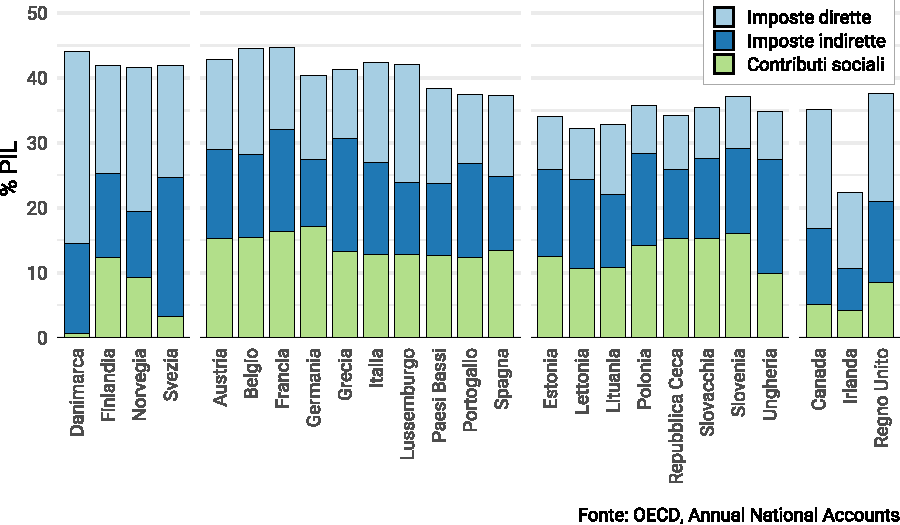
\includegraphics[width=\textwidth]{./figure/classificazione-imposte-oecd-color-2023.pdf}
\end{figure}

\vspace{-3mm}
Il peso delle diverse categorie di imposte nei paesi OCSE (2023)
\end{frame}

%%%%%%%%%%%%%%%%%%%%%%%%%%%%%%%%%%%%%%%%%%%%%%%%%
\begin{frame}{Evoluzione della struttura dei sistemi fiscali nel tempo}
\begin{figure}[htbp]
\centering
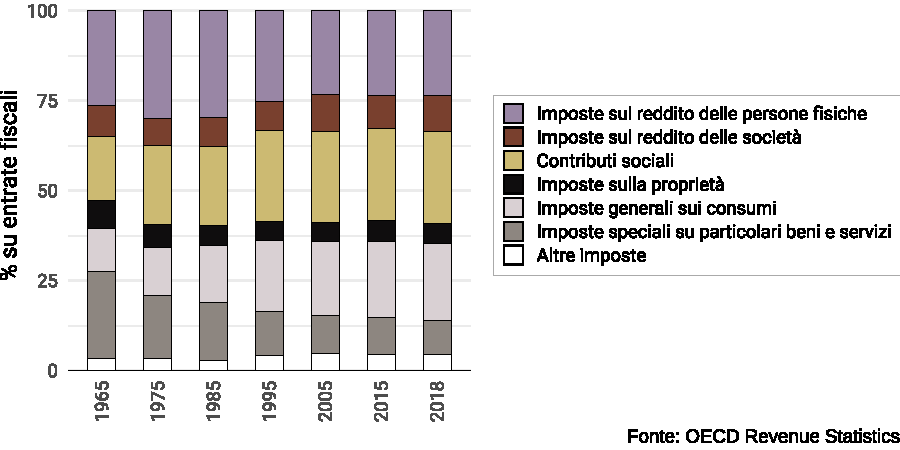
\includegraphics[height=5cm]{./figure/evoluzione-composizione-entrate-OCSE-color.pdf}
\end{figure}

Evoluzione nel tempo:
\begin{itemize}
\item crescita del peso dei contributi sociali;
\item sostituzione di imposte speciali con imposte generali sul consumo (IVA);
\item andamento prima crescente poi decrescente delle imposte sul reddito.
\end{itemize}
\end{frame}

%%%%%%%%%%%%%%%%%%%%%%%%%%%%%%%%%%%%%%%%%%%%%%%%%
\begin{frame}{Le imposte italiane per tipologia e il loro gettito}
\begin{resize}{.7}
\begin{center}
\begin{tabular}{llrr}
 &  &  & mld €\\[0pt]
\hline
imposte & \alert{Irpef} (Imposta sul reddito delle persone fisiche) &  & 221,6\\[0pt]
dirette & \emph{di cui: ritenute su lavoro dipendente e pensioni} & \emph{180,9} & \\[0pt]
erariali & \alert{Ires} (Imposta sul reddito delle società) &  & 51,7\\[0pt]
 & \alert{Isos} (Imposta sostitutiva sui redditi di capitale) &  & 10,0\\[0pt]
 & Altre imposte dirette &  & 34.7\\[0pt]
\hline
imposte & \alert{Iva} (Imposta sul valore aggiunto) &  & 174,9\\[0pt]
indirette & Imposte su prodotti energetici (incl. gas e elettricità) &  & 31,2\\[0pt]
erariali & Lotterie e altri giochi &  & 6,9\\[0pt]
 & Imposta sui tabacchi &  & 11,0\\[0pt]
 & Altre sugli affari (registro, bollo, assicurazione, RAI) &  & 26.5\\[0pt]
\hline
imposte & \alert{Irap} (Imposta regionale sulle attività produttive) &  & 30,1\\[0pt]
locali & \alert{Imu} (Imposta municipale unica) &  & 18,1\\[0pt]
 & \alert{Tasi} (Tassa servizi indivisibili Comuni) &  & 0,1\\[0pt]
 & Addizionali Irpef comunali e regionali &  & 19,5\\[0pt]
 &  &  & \\[0pt]
\end{tabular}
\end{center}
\vspace{-3mm}
{\footnotesize Fonte: \href{https://www.finanze.gov.it/export/sites/finanze/.galleries/Documenti/entrate_tributarie_2023/Bollettino-entrate-Dicembre2023.pdf}{→ Bollettino delle entrate tributarie dic 2023}}
\end{resize}
\begin{itemize}
\item È assente un'imposta patrimoniale erariale di dimensione significativa
(l'imposta di successione svolge un ruolo trascurabile);
\item classificazione tra imposte dirette/indirette dubbia in certi casi: Irap, Imu
\end{itemize}
\end{frame}

%%%%%%%%%%%%%%%%%%%%%%%%%%%%%%%%%%%%%%%%%%%%%%%%%
\begin{frame}{Elementi che descrivono l'imposta}
\begin{resize}{.95}
\begin{itemize}
\item \alert{Soggetto passivo}, su cui ricade l'obbligo di pagamento del
tributo. 
\begin{itemize}
\item Distinguiamo tra \alert{incidenza legale} (chi è giuridicamente è tenuto
  al pagamento dell'imposta) e \alert{incidenza economica} (chi ne sopporta
  effettivamente l'onere);
\item è importante individuare i fattori che determinano la
  \alert{traslazione} dell'imposta da un soggetto all'altro.
\end{itemize}
\item \alert{Presupposto}: il fatto o la circostanza da cui nasce l'obbligo al pagamento
dell'imposta.
\item \alert{Base imponibile}: la grandezza o valore cui si commisura l'imposta, determinata in termini monetari o fisici (imposta \alert{specifica}).
\item \alert{Aliquota}: percentuale o importo da applicare alla base imponibile per
ottenere l'ammontare dell'imposta
\end{itemize}

\begin{block}{}
\alert{Esempio: l'IMU (Imposta Municipale Unica):} Presupposto è il possesso di un'immobile. Soggetto passivo il proprietario o
titolare di diritto reale. Base imponibile è la rendita catastale rivalutata
moltiplicata per un coefficiente a seconda della tipologia
dell'immobile. L'aliquota è 0,40\% nel caso di abitazione principale ecc.
\end{block}
\end{resize}
\end{frame}

%%%%%%%%%%%%%%%%%%%%%%%%%%%%%%%%%%%%%%%%%%%%%%%%%
\begin{frame}{L'aliquota: rapportata a una quantità o ad un valore?}
\begin{itemize}
\item Imposte \alert{specifiche} e \alert{ad valorem}, le prime commisurate alla quantità
fisica, le seconde espresse in percentuale di un valore monetario
\begin{center}
\begin{tabular}{lll}
imposta & gettito & esborso finale\\[0pt]
\hline
specifica & $T = t\cdot q$ & $(p+t)\cdot q$\\[0pt]
\emph{ad valorem} & $T = t\cdot p\cdot q$ & $(1+t)\cdot p\cdot q$\\[0pt]
\end{tabular}
\end{center}
\item Imposte \alert{generali} (esempio: sulla generalità degli scambi) e \alert{speciali}
(sull'acquisto di specifici beni)
\begin{itemize}
\item Le \alert{accise} sono imposte speciali, generalmente specifiche, sul consumo o
la produzione. In Europa sono applicate sugli alcolici, i tabacchi, gli
oli minerali
\end{itemize}
\end{itemize}
\end{frame}

%%%%%%%%%%%%%%%%%%%%%%%%%%%%%%%%%%%%%%%%%%%%%%%%%
\begin{frame}{Imposta su base lorda o su base netta}
\begin{resize}{.95}  
\begin{itemize}
\item Occorre fare attenzione alle aliquote che si applicano sul prezzo al lordo
(\emph{tax inclusive}) o al netto dell'imposta stessa (\emph{tax exclusive})
\begin{itemize}
\item Consideriamo $B_N=B_L-T$
\item l'imposta si può esprimere come percentuale della base lorda (es. imposta sul reddito): $T=\tau_LB_L$, da cui: $B_N=(1-\tau_L)B_L$
\item oppure come percentuale della base netta (es. IVA): $T=\tau_NB_N$, da cui: $B_L=(1+\tau_N)B_N$
\item le due imposte si equivalgono quando $\tau_LB_L=\tau_NB_N$, ovvero:
\end{itemize}
\end{itemize}
\begin{equation*}
\tau_L =\frac{\tau_N}{1+\tau_N} \qquad\tau_N =\frac{\tau_L}{1-\tau_L}.
\end{equation*}
\begin{itemize}
\item Nota bene: i contributi pensionistici sono su base netta per il datore
  di lavoro, su base lorda per il lavoratore.
\end{itemize}
\begin{block}{}
\footnotesize
\alert{ESERCIZIO}. I contributi pensionistici sono commisurati alla retribuzione lorda e sono pari al 23,81\% (su base netta) per il datore di lavoro e al 9,19\% (su base lorda) per il lavoratore. A parità di gettito, quale dovrebbe essere l'aliquota nell'ipotesi di contributi interamente su base lorda o interamente su base netta?
\end{block}
\end{resize}
\end{frame}


%%%%%%%%%%%%%%%%%%%%%%%%%%%%%%%%%%%%%%%%%%%%%%%%%
\begin{frame}{Aliquota media e marginale}
\begin{itemize}
\item \alert{Aliquota media:} definita come il rapporto $T/B$ fra l'imposta e la base imponibile.
\item \alert{Aliquota marginale:} definita come l'imposta che grava su una unità aggiuntiva di base imponibile: $\Delta T/\Delta B$.
\begin{itemize}
\item Ipotizzando che la base imponibile sia una variabile continua e che la
funzione $T(B)$ che descrive l'imposta sia derivabile, l'aliquota
marginale è rappresentata matematicamente dalla derivata prima $T'(B)$.
\end{itemize}
\end{itemize}
\bigskip

\begin{resize}{.9}
\begin{block}{}
\alert{ESEMPIO}. Un'imposta con aliquota del 20\% applicata sulla base imponibile che eccede i 10.000 euro (ovvero in presenza di una deduzione di 10.000 euro).
\begin{itemize}
\item L'aliquota marginale è 20\% al di sopra del 10.000 (è zero al di sotto di tale soglia)
\item L'aliquota media su una base $B$ è $0,2(B-10.000)/B$, dunque è crescente in $B$
\end{itemize}
\end{block}
\end{resize}
\end{frame}


%%%%%%%%%%%%%%%%%%%%%%%%%%%%%%%%%%%%%%%%%%%%%%%%%
\begin{frame}{Il disegno di un sistema fiscale}
Il disegno di un sistema fiscale nasce e si sviluppa in base alla
risposta che viene data ad alcune questioni di fondo:
\begin{itemize}
\item \alert{Chi} deve essere tassato?
\begin{itemize}
\item Gli individui o le famiglie?
\item Solo le persone fisiche o anche le persone giuridiche?
\end{itemize}
\item \alert{Su cosa} e \alert{in che misura} deve essere tassato?\\[0pt]
\begin{itemize}
\item In base all'utilizzo di beni e servizi offerti dalla Pubblica Amministrazione?
\item In base al patrimonio e al reddito? In base ai consumi?
\item Imposte proporzionali a queste quantità? O progressive?
\end{itemize}
\item \alert{Quando} deve essere tassato?  Quando il patrimonio, il reddito, il consumo
si generano o quando si manifestano con flussi finanziari?
\end{itemize}
\end{frame}

\section{Le relazioni tra le imposte}

%%%%%%%%%%%%%%%%%%%%%%%%%%%%%%%%%%%%%%%%%%%%%%%%%
\begin{frame}{Una visione di insieme}
\begin{figure}[htbp]
\centering
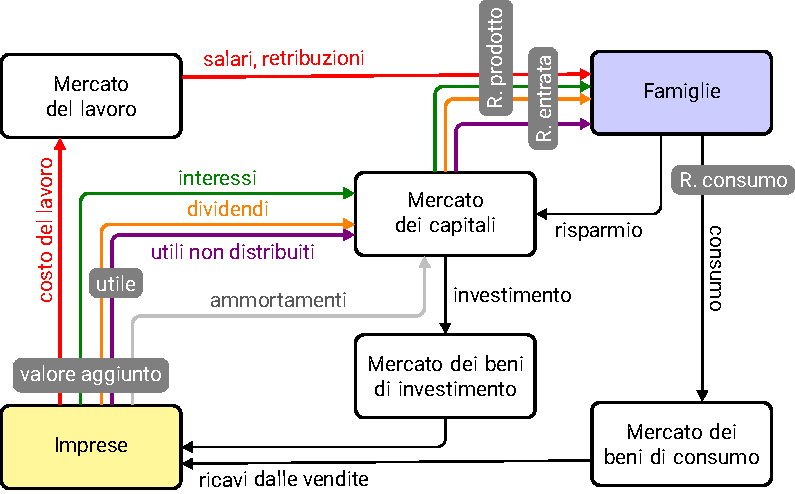
\includegraphics[width=\textwidth]{./figure/flussi-imposte-1.pdf}
\end{figure}
\end{frame}

%%%%%%%%%%%%%%%%%%%%%%%%%%%%%%%%%%%%%%%%%%%%%%%%%
\begin{frame}{L'equivalenza degli effetti delle imposte}
\begin{itemize}
\item Il reddito può essere tassato sul lato delle fonti o su quello degli usi.
\item Come in altri casi, l'effetto può essere valutato con riferimento al vincolo
del consumatore
\item Un'imposta sul reddito: $\sum_ip_ix_i=(1-t)z$.
\item Un'imposta sulla generalità dei consumi (es. IVA): $\sum_i(1+\tau)p_ix_i=z$.
Dividendo:
\begin{equation*}
   \sum_ip_ix_i = \frac{z}{1+\tau}
\end{equation*}
\item C'è equivalenza se:
\begin{equation*}
   1-t = \frac{1}{1+\tau} \quad\text{ovvero: }t = \frac{\tau}{1+\tau}
\end{equation*}
\item Dunque: un'imposta uniforme sui consumi del 20\% equivale a un'imposta
(proporzionale) sul reddito del 16,67\%.
\end{itemize}
\end{frame}


%%%%%%%%%%%%%%%%%%%%%%%%%%%%%%%%%%%%%%%%%%%%%%%%%
\begin{frame}{L'incidenza economica: chi paga realmente un'imposta?}
\begin{itemize}
\item L'analisi dell'incidenza economica individua chi sostiene effettivamente
l'onere economico dell'imposta.
\item Il confronto è tra i \alert{prezzi relativi} di equilibrio con e senza l'imposta:
l'imposta aumenta il prezzo pagato dall'acquirente e riduce il prezzo
ottenuto dal venditore, in misure variabili.
\item Attraverso le variazioni dei prezzi, l'imposta è traslata dal
contributente di diritto \alert{in avanti} (sugli acquirenti del bene), \alert{indietro}
(sui fornitori di fattori produttivi).
\item L'analisi può essere condotta:
\begin{itemize}
\item in \alert{equilibrio parziale}, astraendo dagli effetti che il mutato equilibrio
nel mercato ove è applicata l'imposta determina su altri mercati, e quindi
dai possibili \emph{feedback} sul mercato stesso;
\item in \alert{equilibrio generale}, tenendo conto degli effetti sugli altri mercati.
\end{itemize}
\end{itemize}
\end{frame}

%%%%%%%%%%%%%%%%%%%%%%%%%%%%%%%%%%%%%%%%%%%%%%%%%
\begin{frame}{L'incidenza di un'imposta specifica su un bene di consumo /1}
\begin{columns}
\begin{column}{.5\columnwidth}
\begin{figure}[htbp]
\centering
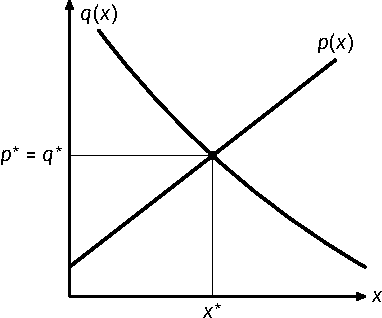
\includegraphics[width=\linewidth]{./figure/incidenza-1.pdf}
\end{figure}
\end{column}


\begin{column}{.45\columnwidth}
In assenza di imposta: chiamiamo $q$ il prezzo per l'acquirente, $p$ il prezzo per il venditore (in funzione della quantità scambiata $x$)
\end{column}
\end{columns}
\end{frame}

%%%%%%%%%%%%%%%%%%%%%%%%%%%%%%%%%%%%%%%%%%%%%%%%%
\begin{frame}{L'incidenza di un'imposta specifica su un bene di consumo}
\begin{columns}
\begin{column}{.5\columnwidth}
Un'imposta $\vartheta$ a carico degli acquirenti

\begin{figure}[htbp]
\centering
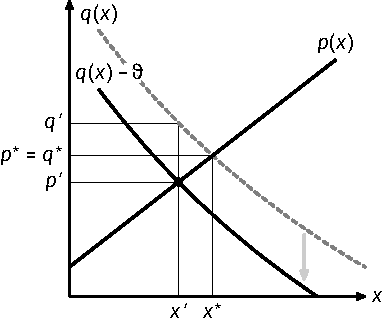
\includegraphics[width=\textwidth]{./figure/incidenza-2.pdf}
\end{figure}
\end{column}

\begin{column}{.5\columnwidth}
Un'imposta $\vartheta$ a carico dei venditori

\begin{figure}[htbp]
\centering
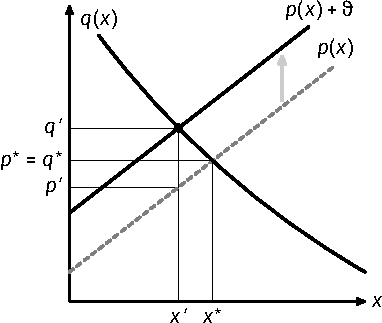
\includegraphics[width=\textwidth]{./figure/incidenza-3.pdf}
\end{figure}
\end{column}
\end{columns}
\medskip
N.B. Lo spostamento delle curve in parallelo caratterizza l'imposta specifica (accisa)
\end{frame}


%%%%%%%%%%%%%%%%%%%%%%%%%%%%%%%%%%%%%%%%%%%%%%%%%
\begin{frame}{Cosa determina l'equilibrio?}
\begin{columns}
\begin{column}{.45\columnwidth}
A parità di $\vartheta$, ai fini degli effetti finali per il venditore e per
l'acquirente, è irrilevante il fatto che l'imposta sia legalmente a carico
dell'uno o dell'altro.
\smallskip

Ciò che conta ai fini della ripartizione del peso dell'imposta è l'elasticità
delle curve di domanda e offerta.
\end{column}

\begin{column}{.5\columnwidth}
\begin{figure}[htbp]
\centering
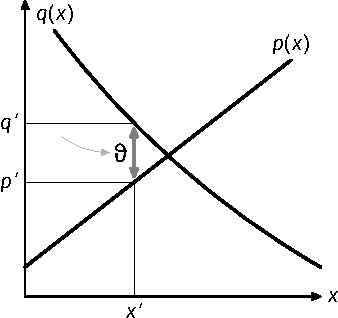
\includegraphics[width=\linewidth]{./figure/incidenza-4.pdf}
\end{figure}
\end{column}
\end{columns}
\end{frame}


%%%%%%%%%%%%%%%%%%%%%%%%%%%%%%%%%%%%%%%%%%%%%%%%%
\begin{frame}{Il ruolo dell'elasticità}
\begin{itemize}
\item Dove ricada il peso dell'imposta dipende
dall'elasticità relativa delle due curve di domanda e offerta;
\item maggiore elasticità significa mobilità e disponibilità di beni sostituti non
tassati, dunque maggiore possibilità di sfuggire all'imposta.
\end{itemize}

\begin{columns}
\begin{column}{.45\columnwidth}
\begin{figure}[htbp]
\centering
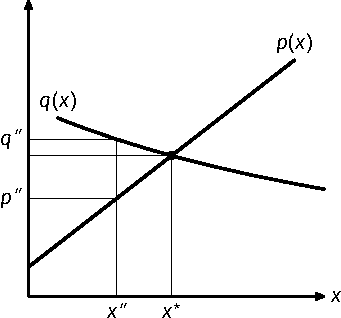
\includegraphics[width=\textwidth]{./figure/incidenza-5.pdf}
\end{figure}
\end{column}

\begin{column}{.45\columnwidth}
\begin{figure}[htbp]
\centering
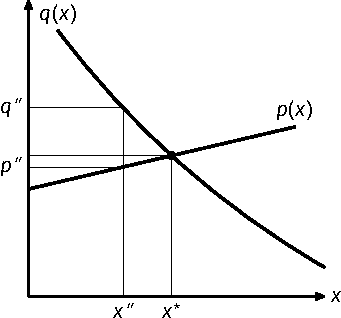
\includegraphics[width=\textwidth]{./figure/incidenza-6.pdf}
\end{figure}
\end{column}
\end{columns}
\end{frame}


%%%%%%%%%%%%%%%%%%%%%%%%%%%%%%%%%%%%%%%%%%%%%%%%%
\begin{frame}{I casi estremi}
\begin{itemize}
\item I casi estremi in cui una delle curve è perfettamente rigida o perfettamente elastica.
\item Esempio di offerta rigida: beni non riproducibili (es. suolo).
  \begin{itemize}
  \item N.B. L'offerta può essere ridida nel breve ma più elastica nel lungo
    periodo.
\end{itemize}
\item Esempio di offerta elastica: un fattore perfettamente mobile.
\end{itemize}

\begin{columns}
\begin{column}{.5\columnwidth}
\begin{figure}[htbp]
\centering
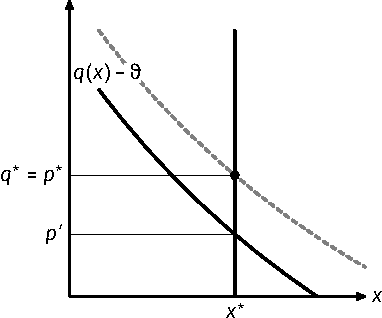
\includegraphics[width=.8\textwidth]{./figure/incidenza-7.pdf}
\end{figure}
\end{column}

\begin{column}{.5\columnwidth}
\begin{figure}[htbp]
\centering
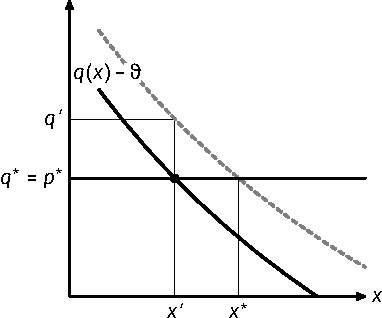
\includegraphics[width=.8\textwidth]{./figure/incidenza-8.pdf}
\end{figure}
\end{column}
\end{columns}
\end{frame}

\section{Perché tanta complessità nei sistemi fiscali?}




%%%%%%%%%%%%%%%%%%%%%%%%%%%%%%%%%%%%%%%%%%%%%%%%%
\begin{frame}{1. Pluralità di obiettivi}
Le principali finalità delle imposte:
\begin{itemize}
\item Gettito per finanziare la spesa.
\item Finalità redistributive.
\end{itemize}
Non bastano le principali imposte (imposta sul reddito e IVA)?
\begin{itemize}
\item Esigenze di gettito immediato (es. imposta sulla benzina utilizzata in più
occasioni per ottenere gettito).
\item Esigenze redistributive, a complemento dell'imposta sul reddito:
\begin{itemize}
\item tassare i beni complementari al tempo libero può essere un modo per
ridurre l'effetto distorsivo dell'imposta sul reddito.
\end{itemize}
\item Imposte finalizzate a correggere esternalità:
\begin{itemize}
\item anche «sin taxes», come imposta su tabacchi, alcolici e \emph{sugar tax}.
\end{itemize}
\item Discriminazione qualitativa dei redditi.
\end{itemize}
\end{frame}

%%%%%%%%%%%%%%%%%%%%%%%%%%%%%%%%%%%%%%%%%%%%%%%%% 
\begin{frame}{2. Vincoli che condizionano il perseguimento degli obettivi}
  \begin{resize}{1.2}
    \begin{itemize}
\item Effetti disincentivanti dell'imposta.
\begin{itemize}
\item Gli effetti disincentivanti delle principali imposte
possono essere attenuati con imposizione mirata su beni
complementari/sostituti rispetto al tempo libero/al lavoro.
\end{itemize}
\item Pianificazione fiscale (\emph{elusione}).
\begin{itemize}
\item Sfrutta le differenze di trattamento fiscale tra diverse tipologie di base
imponibile, tra contribuenti, o dovute alla dimensione della base
imponibile.
\end{itemize}
\item Evasione fiscale.
\end{itemize}
\end{resize}
\end{frame}

%%%%%%%%%%%%%%%%%%%%%%%%%%%%%%%%%%%%%%%%%%%%%%%%%
\begin{frame}{Pianificazione fiscale (elusione)}
\begin{enumerate}
\item Spostare il reddito sui contribuenti con aliquote effettive più basse. Esempi:  
\begin{itemize}
\item l'imprenditore che trasferisce parte del reddito della società al coniuge
  assumendolo come dipendente;
\item il genitore che trasferisce ai figli la proprietà o i diritti reali di
  godimento di attività reali o finanziarie;
\item la società operante in un paese ad alta fiscalità che trasferisce parte
  del proprio reddito alla controllante con sede in un paradiso fiscale.
\end{itemize}
\item Modificare la qualificazione giuridica del reddito:
\begin{itemize}
\item per un contribuente che è contemporaneamente socio e amministratore della
società, il compenso come amministratore è reddito di lavoro mentre la
quota dell’utile è reddito di capitale;
\item interessi, dividendi, plusvalenze.
\end{itemize}
\item Posticipare il momento in cui l’imposta è dovuta.
\end{enumerate}
\end{frame}

%%%%%%%%%%%%%%%%%%%%%%%%%%%%%%%%%%%%%%%%%%%%%%%%% 
\begin{frame}{Il contrasto all'elusione}
\begin{itemize}
\item Con norme specifiche che cercando di limitare specifici abusi.
\item Con soluzioni generali, ad esempio GAAR (\emph{general anti-abuse
    rule}), richieste in UE della Anti Tax Avoidance Directive del 2016.
\item In Italia sono considerate elusione e quindi sanzionate le «operazioni
  prive di sostanza economica che, pur nel rispetto formale delle norme
  fiscali, realizzano essenzialmente vantaggi fiscali indebiti.»
\begin{itemize}
\item Sono \alert{operazioni prive di sostanza economica} «i fatti, gli atti
e i contratti, anche tra loro collegati, inidonei a produrre effetti
significativi diversi dai vantaggi fiscali»
\item Sono \alert{vantaggi fiscali indebitamente conseguiti} «i benefici, anche non
immediati, realizzati in contrasto con le finalità delle norme fiscali o
con i principi dell'ordinamento tributario.»
\item Non si considerano invece elusive «le operazioni giustificate da valide
ragioni extrafiscali non marginali, anche di ordine organizzativo o
gestionale, che rispondono a finalità di miglioramento strutturale o
funzionale dell'impresa o dell'attività professionale del contribuente.»
\end{itemize}
\end{itemize}
\end{frame}

%%%%%%%%%%%%%%%%%%%%%%%%%%%%%%%%%%%%%%%%%%%%%%%%%
\begin{frame}{L'evasione fiscale}
  \begin{itemize}
\item Si definisce evasione un comportamento \emph{illegale} mirante a ridurre o eliminare il prelievo fiscale (ad es. omessa o infedele dichiarazione).
\item L'entità dell'evasione in Italia è quantificata nella \emph{Relazione
    sull'economia non osservata e sull'evasione fiscale e contributiva}
  redatta da una commissione del MEF.
\item Indicatore utilizzato è il \emph{tax gap}, differenza tra gettito e gettito
«teorico»
\end{itemize}

\begin{center}
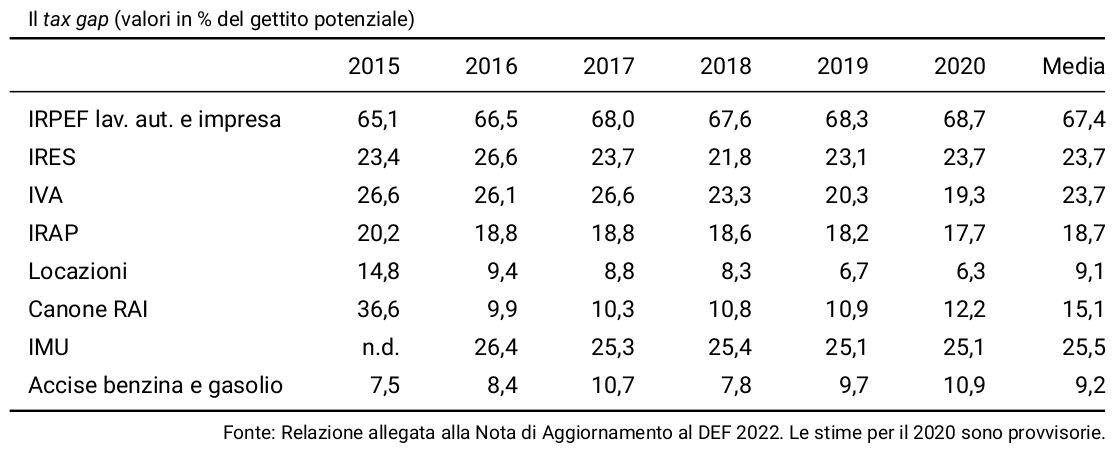
\includegraphics[width=.9\linewidth]{./figure/tax-gap.png}
\end{center}  
\end{frame}

%%%%%%%%%%%%%%%%%%%%%%%%%%%%%%%%%%%%%%%%%%%%%%%%%
\begin{frame}{Evasione fiscale: analisi formale}
Semplice modello di scelta razionale
\begin{itemize}
\item $z$ reddito effettivo e $\hat{z}$ reddito dichiarato, con $0\le\hat{z}\le z$
\item $\pi$ probabilità di accertamento; l'accertamento comporta una sanzione
$\gamma$ proporzionale al reddito evaso $z-\hat{z}$
\item Dunque, evadere è una scommessa:
\begin{itemize}
\item in caso di accertamento il reddito netto del contribuente sarà $x_A=(1-t)z-t\gamma(z-\hat z)$;
\item senza accertamento, sarà $x_N=z-t\hat{z} = (1-t)z+t(z-\hat z)$.
\item se neutrale al rischio, sceglie $\hat z$ per massimizzare: $\pi x_A + (1-\pi) x_N$;
\item se avverso al rischio sceglie $\hat z$ in modo da massimizzare l'utilità attesa: $\pi
    u(x_A)+(1-\pi)u(x_N)$.
\end{itemize}
\end{itemize}
\end{frame}

%%%%%%%%%%%%%%%%%%%%%%%%%%%%%%%%%%%%%%%%%%%%%%%%%
\begin{frame}{Evasione fiscale: analisi formale /2}
\begin{columns}
\begin{column}{.45\columnwidth}
\begin{itemize}
\item Con $\hat{z}=z$ abbiamo: $x_N(z)=x_A(z)=(1-t)z$;
\item con $\hat{z}=0$ abbiamo $x_N(0)=z$ e $x_A(0)=(1-t(1+\gamma))z$;
\item al variare di $\hat{z}$ individuiamo il vincolo di espressione $x_N=(1-t)(1+\gamma)z-\gamma x_A$\\
  (il segmento in figura);
\item ottimale non evadere se
$$ -\text{SMS}=-\frac{1-\pi}{\pi} >-\gamma $$
cioè se $\gamma$ o $\pi$ sono sufficientemente elevati.
\end{itemize}
\end{column}
\begin{column}{.55\columnwidth}
\begin{center}
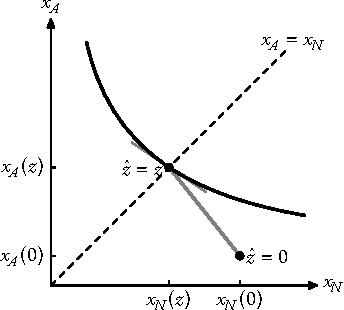
\includegraphics[width=\textwidth]{./figure/evasione-1.pdf}
\end{center}
\end{column}
\end{columns}
\end{frame}


%%%%%%%%%%%%%%%%%%%%%%%%%%%%%%%%%%%%%%%%%%%%%%%%%
\begin{frame}{Evasione fiscale: analisi formale /3}
\begin{columns}
\begin{column}{.45\columnwidth}
\begin{itemize}
\item Se invece $\gamma$ e $\pi$ tali che:
$$ -\text{SMS}=-\frac{1-\pi}{\pi} <-\gamma $$
l'equilibrio è in E dove
\begin{equation*}
 -\text{SMS} = -\frac{u'(x_N)}{u'(x_A)}\frac{1-\pi}{\pi}=-\gamma.
\end{equation*}
\item Quale l'effetto di $z$ e $t$?\\ Un aumento di $t$ e una riduzione di $z$ spostano verso il basso il vincolo di bilancio lasciando invariata la pendenza.
  \item Non è dunque ovvio, dal modello, che un aumento di $t$ aumenti l'evasione.
\end{itemize}
\end{column}
\begin{column}{.55\columnwidth}
\begin{center}
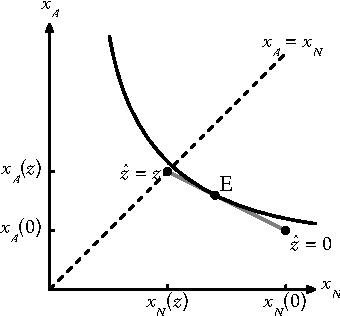
\includegraphics[width=\textwidth]{./figure/evasione-2.pdf}
\end{center}
\end{column}
\end{columns}
\end{frame}

%%%%%%%%%%%%%%%%%%%%%%%%%%%%%%%%%%%%%%%%%%%%%%%%%
\begin{frame}{Ruolo delle sanzioni}
\begin{itemize}
\item L'esperienza italiana non sembra confermare la tesi che sanzioni elevate
sono un deterrente efficace
\item Attualmente:
\begin{itemize}
\item sanzioni penali in alcuni casi (omessa dichiarazione se ammontare evaso
superiore a 50 mila euro, dichiarazione infedele se ammontare supera i 150
mila euro, omesso versamento di ritenute\ldots{})
\item sanzione amministrativa (la sanzione varia tra il 120\% e il 240\%
dell'imposta non versata, con minimo di 250 €)
\end{itemize}
\item Più controlli? I controlli sono costosi, non sempre danno luogo al recupero
della somma evasa, può portare a contenzioso ecc. e alla fine del percorso
il contribuente potrebbe non avere risorse per pagare
\item Ultimamente strumenti preventivi:
\begin{itemize}
\item ruolo di «terze parti»
\item ricorso a ritenute (es. redditi di capitale prelevati dagli intermediari
finanziari)
\end{itemize}
\end{itemize}
\end{frame}

\begin{frame}
  \frametitle{3. La natura incrementale delle riforme fiscali}

  \begin{resize}{1.1}
    \begin{itemize}
    \item Un'ulteriore fonte di complessità è la stratificazione di riforme che
      possono rispondere a visioni differenti o a esigenze contingenti.
    \item Difficile realizzare operazioni di razionalizzazione o di riforma
      complessiva del sistema fiscale.
    \end{itemize}
  \end{resize}
\end{frame}

\section{L'evoluzione del sistema fiscale italiano}

%%%%%%%%%%%%%%%%%%%%%%%%%%%%%%%%%%%%%%%%%%%%%%%%%
\begin{frame}{Il peso delle diverse categorie di imposta: evoluzione 1965-2020}
\begin{center}
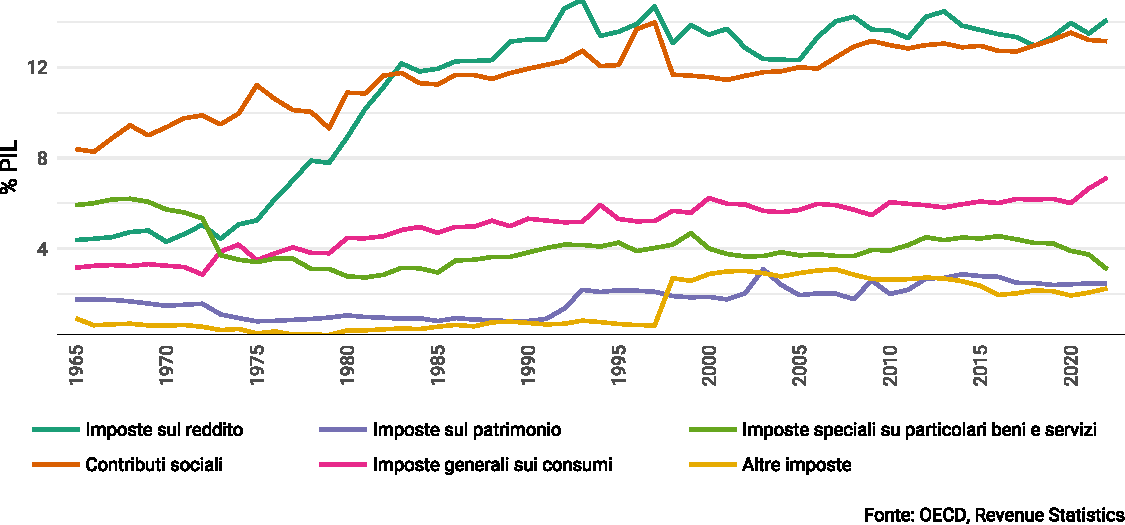
\includegraphics[width=\textwidth]{./figure/evoluzione-struttura-imposte-ITA-2022-color.pdf}
\end{center}
\end{frame}

\begin{frame}{Le riforme fiscali dagli anni Sessanta in poi}
  \begin{description}
  \item[Anni Sessanta:] prevalenza delle imposte indirette, tra cui l'IGE; imposte dirette in prevalenza reali (imposta di ricchezza mobile); imposte fondiarie; imposta complementare progressiva sul reddito.
\smallskip
    Istituita la «Commissione Cosciani» per elaborare una riforma complessiva del sistema fiscale.
    
  \item[Anni Settanta:] riorganizzazione del sistema fiscale, attorno a IRPEF,
    IRPEG e IVA. Imposte introdotte nel 1973-1974; acquistano preminenti le
    imposte dirette personali e le imposte indirette generali rispetto a
    quelle speciali.

    Aumento del gettito dell'IRPEF negli anni successivi, per effetto anche
    dell'inflazione e del \emph{fiscal drag}.
  \end{description}
\end{frame}

\begin{frame}{Le riforme fiscali dagli anni Sessanta in poi /2}
  \begin{description}
    
  \item[Anni Novanta e primi Duemila:] nuove sfide poste dalla liberalizzazione dei movimenti di capitale in un contesto di riduzione delle imposte a livello internazionale. Due fasi di riforma:
    \begin{itemize}
    \item Riforma Visco (1997): obiettivi di semplificazione, neutralità nelle
      scelte di investimento, ampiamento della base imponibile. Realizzati
      attraverso l'armonizzazione delle aliquote sui redditi di capitale, la
      tassazione delle plusvalenze, l'introduzione dell'IRAP, la tassazione
      duale del reddito societario.
    \item Riforme Berlusconi-Tremonti (2001-2004): depotenziamento e abolizione di alcune delle novità introdotte dalla riforma Visco; riforma tassazione societaria (IRES). 
    \end{itemize}
  \item[Dal 2010 in poi:] In conseguenza della crisi finanziaria e delle politiche di austerità, aumento del prelievo (specialmente su immobili e IVA); interventi su categorie individuali di reddito, proliferazione dei regimi sostitutivi.
    
  \end{description}

\end{frame}

\end{document}